\documentclass[a4paper,american]{lipics-v2016}
%\usepackage[USenglish]{babel}
%\usepackage{microtype}
\bibliographystyle{plainurl}
\title{One exact and one random sampling method to assess the reliability of inferences from network enrichment analysis}
\titlerunning{Null models for Network Enrichment Analysis} %optional, in case that the title is too long; the running title should fit into the top page column

%% Please provide for each author the \author and \affil macro, even when authors have the same affiliation, i.e. for each author there needs to be the  \author and \affil macros
\author[1]{Gustavo S. Jeuken}
\author[2]{Lukas K\"{a}ll}
\affil[1]{Science for Life Laboratory, School of
Engineering Sciences in Chemistry, Biotechnology and Health,
Royal Institute of Technology -- KTH, Box 1031, 17121 Solna, Sweden\\ \texttt{gustavo.jeuken@scilifelab.se}}
\affil[2]{Science for Life Laboratory, School of
Engineering Sciences in Chemistry, Biotechnology and Health,
Royal Institute of Technology -- KTH, Box 1031, 17121 Solna, Sweden\\ \texttt{lukas.kall@scilifelab.se}}
\authorrunning{G. S. Jeuken and L. K\"{a}ll}

\Copyright{Gustavo S. Jeuken and Lukas K\"{a}ll}%mandatory, please use full first names. LIPIcs license is "CC-BY";  http://creativecommons.org/licenses/by/3.0/

\subjclass{G.3. Probabilistic algorithms (including Monte Carlo)}% mandatory: Please choose ACM 1998 classifications from http://www.acm.org/about/class/ccs98-html . E.g., cite as "F.1.1 Models of Computation".
\keywords{Gene Set Analysis; Calibration; Null model; p value; Sampling}% mandatory: Please provide 1-5 keywords



%Editor-only macros:: begin (do not touch as author)%%%%%%%%%%%%%%%%%%%%%%%%%%%%%%%%%%
%\EventEditors{John Q. Open and Joan R. Acces}
%\EventNoEds{2}
\EventLongTitle{18th Workshop on Algorithms in Bioinformatics (WABI 2018)}
\EventShortTitle{WABI 2018}
\EventAcronym{WABI}
\EventYear{2018}
\EventDate{20–22 August 2018}
\EventLocation{Helsinki, Finland}
%\EventLogo{}
%\SeriesVolume{42}
%\ArticleNo{23}
% Editor-only macros::end %%%%%%%%%%%%%%%%%%%%%%%%%%%%%%%%%%%%%%%%%%%%%%%



\begin{document}

\maketitle

\begin{abstract}
A prevailing technique to infer function from identifications from molecular biological high-throughput experiments is gene set enrichment analysis, where the identifications are compared to predefined sets of related genes, so-called pathways. As at least some pathways are known to be incomplete in their annotation, algorithmic efforts have been made to complement them with information from functional association networks, with so-called Network Enrichment Analysis (NEA). Traditionally, the significance of inferences from NEA has been assigned using parametric models, that are tuned by fitting parameters by sampling random network perturbations. Here we instead have designed one dynamic programming  algorithm that calculates the score distribution of NEA scores and makes it possible to assign unbiased mid $p$~values to inferences. We also implemented a random sampling method, carrying out the same task. We demonstrate that our method obtains a superior statistical calibration as compared to the popular NEA inference engine, BinoX.

\end{abstract}

\section*{Introduction}

Gene enrichment analysis (GEA) is commonly used to infer function from sets of analytes such as genes, transcripts proteins or metabolites\cite{tavazoie1999systematic,khatri2012ten}. The technique estimates which functional modules, such as complexes or pathways, that are overrepresented among a set of identified analytes. One prominent application of the technique is expression analysis, where GEA is regularly used to assess alternation in pathway activity by examining significantly different concentrations of analytes between biological conditions, such as disease state or treatment group.

Most GEA methods are assessing the overlap between the investigated set of analytes, the {\em query set}, and a functional module, the {\em pathway set}, using hypergeometric test or a Fisher's exact test. However, variants such as Gene Set Enrichment Analysis (GSEA)\cite{subramanian2005gene} also includes information on expression levels of the analytes of the query set.

A limiting factor of GEA is the pathway definition databases. While \url{http://pathguide.org} list 708 databases of pathway definitions\cite{bader2006pathguide},  some critique has been voiced concerning the completeness and rigor of current pathway databases. Hence efforts have been directed to designing methods that extend the pathway definitions, by functional association networks, like STRING\cite{szklarczyk2014string} and FunCoup\cite{ogris2017funcoup}. Instead of directly examining the overlap between the query and pathway sets, one can evaluate the number of links in the functional association network that connect the query and pathway set\cite{alexeyenko2012network, glaab2012enrichnet, mccormack2013statistical, ogris2016novel, signorelli2016neat}. This is known as Network Enrichment Analysis (NEA).

The significance of the inferences from NEA is assessed by null models that investigate the number of expected random links from the query gene set to the pathway. Previous efforts have settled for various parametric null distributions, where the parameters are estimated by Monte Carlo-simulations that permute the network definitions by methods with varying degrees of topological conservation.

As it is difficult to design network randomization techniques that are completely random, such methods often introduce an undesirable bias in the statistics. For instance, the actual set of random networks is much larger than the ones one use in such test, namely the random networks that retain a certain topological characteristic\cite{newman2001random}. Also, the somewhat inaccessible process used to randomize networks produces statistics that are equally hard to interpret, as such statistic in practice test a more complex null model than intended.

Users of NEA typically want to test if there is a functional association between a query set of genes and a pathway\cite{alexeyenko2012network}. We argue that such test are much easier implemented as tests of the query set, i.e. is the query set a randomly selected set of genes, or is there an overrepresentation of well-connected genes in the query set?

Hence, here we employ a different null model, more directly aimed at model lack of association between query and pathway gene sets, which we formulate as ``there are not more links between the query and pathway gene sets than expected by chance''. We present a dynamic programming algorithm, that we dubbed GeneSetDP, that calculates the exact score distribution of any query of a given size. We also implemented one random sampling algorithm for the same task, that we called GeneSetMC.
The algorithms enabled us to calculate well-defined statistics of inferences from NEA.  Using simulations we demonstrated that both the algorithms produced unbiased statistics.

\section*{Algorithms}

In network-based gene set analysis one score a query set of genes $ \mathcal{Q}=\{g_1 \ldots g_Q\} $ from a genome with genes $\mathcal{G}=\{g_1 \ldots g_G\}$ ($Q \le G$), and how they relate to a pathway $\{p_1 \ldots p_P\}$. In NEA the pathway maps to the genome through a network ${x_{ij}}$, where $x_{ij}=1$ if $g_i$ and $p_j$ are connected, or $x_{ij}=0$ otherwise. The pathways are scored by summing up all connections, i.e. the pathway score is

\begin{equation}
s=\sum_{i=1}^Q\sum_{j=1}^P x_{ij}.
\label{eq:sum_ij}
\end{equation}

Here, we wanted to determine a score distribution, {\em i.e.} the number of ways, $N(s)$, we can pick $Q$ genes and obtaining a score, $s$. This allows us to evaluate our score against the null hypothesis, $H_0$ : ``There are not more links between the query and pathway gene sets than expected by chance''. This translates to evaluate yje distribution of scores that would occure if the $Q$ query genes are randomly selected from the genome''. This can be expressed as a mid $p$~value\cite{lancaster1961significance,hwang2001optimality} for obtaining a score $s$,

\begin{equation}
p(s)=\frac{N(s)/2 +\sum_{s'=s+1}^{S} N(s')}{\sum_{s'=0}^{S} N(s')},
\label{eq:pval}
\end{equation}
where $S$ is the maximal score $s$ that $Q$ genes can obtain from Equation \ref{eq:sum_ij}.

We can reformulate Equation \ref{eq:sum_ij} by defining the number-of-links, $l_i=\sum_{j=1}^P x_{ij}$, which gives us a score,
\begin{equation}
s=\sum_{i=1}^Q l_i.
\label{eq:sum_i}
\end{equation}
Such number-of-links, $l_i$, can be pre-computed for all genes $i, \ldots, G$.

\subsection*{Random sampling algorithm}

We first implemented a random sampling algorithm to assess $N(s)$. We randomly selected sets of $Q$ genes from $\mathcal{G}$. These sets scores were calculated with Equation \ref{eq:sum_i}. We counted the number of times $F_B(s)$ a score of $s$ was obtained when sampling $B$ gene sets. We see that $F_B(s)$ will approximately have the same shape as $N(s)$ when selecting a large $B$, and we can hence calculate $p$~values by replacing $N$ with $F_B$ in Equation~\ref{eq:pval}. We refer to this procedure as GeneSetMC.

\subsection*{Computation of the score distribution}

Furthermore, the number of genes having $a$ links to the investigated pathway is given by $k_a=\sum_{\{i:l_i=a\}}1$, and $R=\max_{i}{l_i}$.

In our strive to calculate the score distribution, $N(s)$, we first want to investigate the number of ways, $N_a(s,c)$, to obtain a score $s$, when summing up links for $c$ genes with up to $\le a$ links to the pathway. This helps us formulate the recursion, using the fact that there are $k_a \choose b$ ways to select $b$ from $k_a$ elements, as
\begin{equation}
N_a(s,c)=\sum_{b=0}^{k_a}{k_a \choose b} N_{a-1}(s-ab,c-b),
\end{equation}
where $N_a(s,c)=0$ for all $s<0$, $c<0$ or $a<0$, with the exception for $N_{-1}(0,0)=1$.

The final score distribution is given by $N(s)=N_R(s,Q)$.

\subsection*{Implementation}

\begin{lstlisting}[caption={
The central part of the dynamic programing algorithm for finding $N(s)$. The function takes the vector of links per gene, $k_a$, as well as the number of query genes, $Q$ as an input. The function depends on two additional functions {\tt find\_maxscore(k,Q)}, which calculates the maximal score a query of size $Q$ can obtain, and {\tt comb(a,b)}, which calculates $ a \choose b $.
}
, label=lst:gensetdp,captionpos=t,float,abovecaptionskip=-\medskipamount]
def genesetdp(k,Q):
    max_s = find_maxscore(k,Q)
    N = np.zeros((max_s+1,Q+1))
    N[0,0] = 1

    for a in range(len(k)):
        for s in range(max_s,-1,-1):
            for c in range(Q,-1,-1):
                for b in range(k[a],0,-1): # Stop at b=1
                    if c-b>=0 and s-a*b>=0:
                        N[s,c] += comb(k[a], b) * N[s-a*b,c-b]
    return N[:,q]
\end{lstlisting}
There is a memory efficient implementation. We first note that

\[
N_a(s,c)=\sum_{b=1}^{k_a}{k_a \choose b} N_{a-1}(s-ab,c-b) + N_{a-1}(s,c)=D_a+N_{a-1}(s,c).
\]


This enables us to calculate $N$ in-place, at least as long as we update the elements in $N_a$ in a reverse order so that we do not alter elements from $N_{a-1}$ still needed to update subsequent elements. That is, we do not have to copy the dynamic programming matrix in each iteration over $a$, instead, we can add a $D_a$ on to of previous iterations $N_{a-1}(s,c)$, by nested updates over $s \in \{ RQ, RQ-1, \ldots 0 \}$ and $c \in \{ Q, Q-1, \ldots 1 \}$. For details see Listing \ref{lst:gensetdp}. We refer to this method as GeneSetDP.

\section*{Methods}

We downloaded network definitions and the BinoX software (on 2018-04-28) for comparisons from \url{https://bitbucket.org/sonnhammergroup/binox}. BinoX was run with the default parameters.
% FIXME: add a more detailed description of the test set (i.e. organism and number of genes, pathways and network connections).

We also downloaded the NEA example given at the BinoX web site. The example files include a pathway definition file that groups $6819$ genes into $289$ human pathways and a network definition file that, after thresholding with a score of $0.7$, gave $1244992$ links between those genes.

For the purpose of demonstrating our argument, we selected a representative example in the ``Glycolysis/Gluconeogenesis'' pathway, as it contained a number of genes that coincided with the median number of genes of the pathways in the definition file.

\subsection*{Availability}

Source code of an implementation of GeneSetDP and GeneSetMC, as well as code for generating the plots of this paper, is available from \url{https://github.com/statisticalbiotechnology/genesetdp}.

\section*{Results}

We implemented a Python program that reads network and pathway definition files and scores a query sets against a pathway according to Equation \ref{eq:sum_i}, using GeneSetDP and GeneSetMC described in the Algorithm section, that enabled us to assign $p$~values according to Equation \ref{eq:pval}. We downloaded pathway and network definitions from the BinoX's website and used the same network threshold as BinoX default ($0.7$).

To illustrate the $p$~value calculation procedure, we plotted the score distributions $N(s)$ for a query size of 10, 20 and 30 genes in Figure \ref{fig:score_dist}, using GeneSetDP.

\begin{figure}[htb]
	\begin{center}
		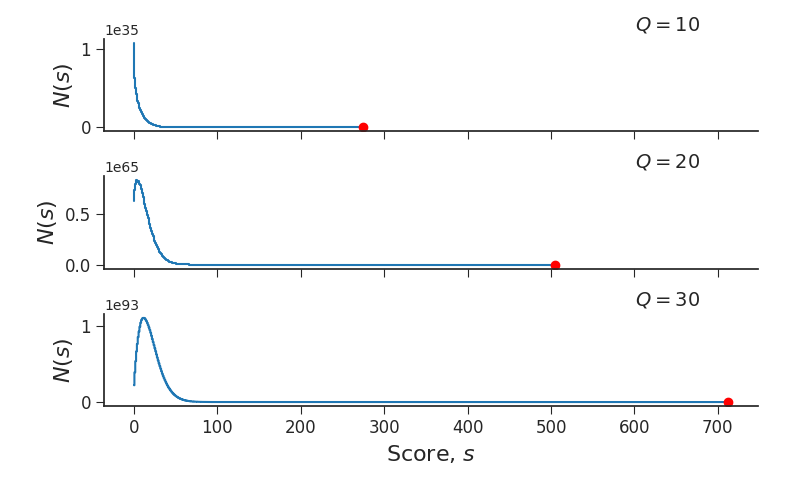
\includegraphics[width=1.0\textwidth]{figures/score_distribuition_multiple.png} 
    \end{center}
  \caption{{\bf Score distribution of a query size of 10, 20 and 30 genes against the ``Glycolysis/Gluconeogenesis'' pathway.} GeneSetDP enables us to calculate the full score distribution for a query of a given size, $Q$, i.e. how many ways one can reach a certain score when adding up the scores for $Q$ genes.}
  \label{fig:score_dist}
\end{figure}

\subsection*{Test of Calibration}

In order to test the statistical calibration of our method, we calculated $p$~values for 10000 random picks of gene sets from the investigated genome. As our selection is random and following our null hypothesis, we expected the resulting $p$~values to be uniformly distributed. To test this we plotted the $p$~values against their quantile in Figure \ref{fig:calibration} for $10000$ randomly assembled queries from the human genome. As a comparison, we also added a calibration curve for the popular NEA method BinoX\cite{ogris2016novel}.

We note that the calibration of GeneSetDP is slightly conservative, i.e. the calculated $p$ values are larger than expected. Meanwhile, BinoX appears strongly anti-conservative, that is, the $p$ values are lower than expected.

\begin{figure}[htb]
  \begin{center}
		  \begin{tabular}[t]{c}
				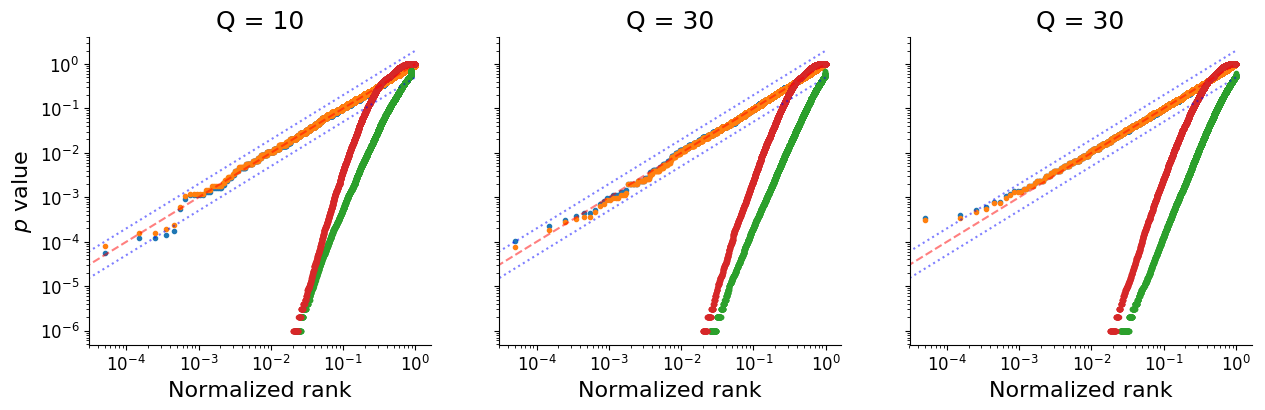
\includegraphics[width=1.0\textwidth]{figures/calibration_multiple.png} \\
				
\includegraphics[width=0.5\textwidth]{figures/calibration_legend.png}
		\end{tabular}
  \end{center}
  \caption{{\bf Calibration of GeneSetDP and GeneSetMC.} We selected 10000 random sets of 10, 20 and 30 genes from the investigated genome definition and calculated their $p$ values with GeneSetMC and GeneSetDP against the ``Glycolysis/Gluconeogenesis'' pathway. To test the $p$~values uniformity we plotted them against their {\em normalized rank}, i.e. each $p$~value's (<rank>-0.5)/<total number of $p$~values>. We also added the calibration curve of BinoX, evaluated on the same random sets. On all plots the dashed line shows $y = x$ and the dotted lines $y = 2x$ and $y = 0.5x$, for comparison}
  \label{fig:calibration}
\end{figure}


\section*{Discussion}

Here we have implemented two methods, GeneSetDP and GeneSetMC, to calculate unbiased $p$~values for inferences from NEA.
Instead of testing our methods performance in terms of sensitivity, we here instead chose to test the method in terms of the methods statistical accuracy. We argue that more studies should make a point at demonstrate that their methods are well calibrated, as it is a prerequisite for measuring performance at least when ground truth of biological effect is not known.
With this in mind, we demonstrated that our methods gave a better calibration than the popular BinoX method, by random sampling of subsets of a genome.

Both our implementations, GeneSetDP and GeneSetMC, are intended for measuring enrichment of links between the query and the pathway set of genes. Most other NEA methods also report depletion of such links. One could easily modify our code to instead of only measuring the higher scoring tail measuring both tails of $N(s)$. However, this might result in a drop in sensitivity, so we have so far no implemented such a mechanism.

Here we made an explicit definition of the null hypothesis we employed, which centers on the query, $H_0$ : ``There are not more links between the query and pathway gene sets than expected by chance''. Previous implementations of NEA in the literature use Monte Carlo-simulation to determine parameters for various types parametric distributions, by perturbations of the investigated network. In practice, such perturbations are hard to conduct in a manner that they still resemble the original network, and hence are difficult to use to calculate accurate statistics. In general, it is easier to understand null models that relate to user actions, than more complex null models that relate to model parameters.

\bibliography{./refs}

\end{document}
